%% defense.tex
%% Copyright 2022 Tom M. Ragonneau
%
% This work may be distributed and/or modified under the
% conditions of the LaTeX Project Public License, either version 1.3
% of this license or (at your option) any later version.
% The latest version of this license is in
%   http://www.latex-project.org/lppl.txt
% and version 1.3 or later is part of all distributions of LaTeX
% version 2005/12/01 or later.
%
% This work has the LPPL maintenance status `maintained'.
%
% The Current Maintainer of this work is Tom M. Ragonneau.
\documentclass{polyu-presentation}
\usepackage{microtype}
\usepackage{booktabs}

% List of hyphenation exceptions for US English
% Source: https://ctan.org/tex-archive/info/digests/tugboat/hyphenex
\input{ushyphex}

% Bibliographical resources
\addbibresource{ragonneau-bib/strings.bib}
\addbibresource{ragonneau-bib/optim.bib}

% Dedicated mathematical macros
\usepackage{xargs}
\newcommand{\auglag}{\mathcal{L}_{\mathsf{A}}}
\newcommand{\auglagalt}{\widetilde{\mathcal{L}}_{\mathsf{A}}}
\newcommand{\con}[1][]{c\ifthenelse{\equal{#1}{}}{}{_{#1}}}
\newcommandx{\conm}[2][1={},2={}]{\hat{c}\ifthenelse{\equal{#2}{}}{}{_{#2}}\ifthenelse{\equal{#1}{}}{}{^{#1}}}
\newcommand{\fset}{\Omega}
\newcommand{\ieq}{\mathcal{E}}
\newcommand{\iub}{\mathcal{I}}
\newcommand{\iter}[1][]{x\ifthenelse{\equal{#1}{}}{}{^{#1}}}
\newcommand{\lag}[1][]{\mathcal{L}\ifthenelse{\equal{#1}{}}{}{^{#1}}}
\newcommand{\lagalt}[1][]{\widetilde{\mathcal{L}}\ifthenelse{\equal{#1}{}}{}{^{#1}}}
\newcommand{\lagm}[1][]{\hat{\mathcal{L}}\ifthenelse{\equal{#1}{}}{}{^{#1}}}
\newcommand{\lagp}[1][]{L\ifthenelse{\equal{#1}{}}{}{_{#1}}}
\newcommand{\lm}[1][]{\lambda\ifthenelse{\equal{#1}{}}{}{^{#1}}}
\newcommand{\lpoly}{\mathscr{L}(\R^n)}
\newcommand{\merit}[1][]{\varphi\ifthenelse{\equal{#1}{}}{}{^{#1}}}
\newcommand{\meritm}[1][]{\hat{\varphi}\ifthenelse{\equal{#1}{}}{}{^{#1}}}
\newcommand{\nstep}[1][]{n\ifthenelse{\equal{#1}{}}{}{^{#1}}}
\newcommand{\nstepalt}[1][]{\bar{n}\ifthenelse{\equal{#1}{}}{}{^{#1}}}
\newcommand{\obj}{f}
\newcommand{\objm}[1][]{\hat{f}\ifthenelse{\equal{#1}{}}{}{^{#1}}}
\newcommand{\objmalt}[1][]{\tilde{f}\ifthenelse{\equal{#1}{}}{}{^{#1}}}
\newcommand{\pstep}[1][]{p\ifthenelse{\equal{#1}{}}{}{^{#1}}}
\newcommand{\qpoly}{\mathscr{Q}(\R^n)}
\newcommand{\rad}[1][]{\Delta\ifthenelse{\equal{#1}{}}{}{@\!^{#1}}}
\newcommand{\radlb}[1][]{\delta\ifthenelse{\equal{#1}{}}{}{^{#1}}}
\newcommand{\ratio}[1][]{\rho\ifthenelse{\equal{#1}{}}{}{^{#1}}}
\newcommand{\rstep}[1][]{r\ifthenelse{\equal{#1}{}}{}{^{#1}}}
\newcommand{\sstep}[1][]{s\ifthenelse{\equal{#1}{}}{}{^{#1}}}
\newcommand{\step}[1][]{d\ifthenelse{\equal{#1}{}}{}{^{#1}}}
\newcommand{\tstep}[1][]{t\ifthenelse{\equal{#1}{}}{}{^{#1}}}
\newcommand{\xl}{l}
\newcommand{\xpb}[1][]{\mathcal{P}}
\newcommand{\xpt}[1][]{\mathcal{Y}\ifthenelse{\equal{#1}{}}{}{^{#1}}}
\newcommand{\xsv}[1][]{\mathcal{S}}
\newcommand{\xu}{u}

% If-Then-Else function for pgfplots
\pgfmathdeclarefunction{ifthenelsefpu}{3}{\pgfmathparse{#1*#2 + !#1*#3}}

% Performance and data profiles
\usepackage{xstring}
\newcommand{\drawprofiles}[4]{%
    \def\selectsolvers{#2}%
    \def\selectcsv{figures/#3}%
    \def\selectprofile{#4}%
    \ifthenelse{\equal{#1}{performance}}{%
        \def\selectxlabel{$\log_2(\text{perf.\ ratio})$}%
        \def\selectylabel{Perf.\ profiles ($\tau = 10^{-#4}$)}%
    }{%
        \def\selectxlabel{Number of simplex gradients}%
        \def\selectylabel{Data profiles ($\tau = 10^{-#4}$)}%
    }
    \input{figures/profiles.tex}%
}
\newcommand{\drawperformanceprofiles}[3]{\drawprofiles{performance}{#1}{#2}{#3}}
\newcommand{\drawdataprofiles}[3]{\drawprofiles{data}{#1}{#2}{#3}}

\title{Model-Based DFO Methods and Software}
\subtitle{Ph.D. thesis defense}
\author[Tom M. Ragonneau]{\texorpdfstring{
    Tom M. Ragonneau\\
    \footnotesize Co-supervised by Dr.\ Zaikun Zhang and Prof.\ Xiaojun Chen
}{Tom M. Ragonneau}}
\institute[PolyU AMA]{
    Department of Applied Mathematics\\
    The Hong Kong Polytechnic University
}
\date{December 6, 2022}
\titlegraphic{\href{https://www.tomragonneau.com/}{\includegraphics[width=0.8in]{images/qr/personal.png}}}

\begin{document}

\begin{frame}
	\titlepage
\end{frame}

\begin{frame}
    \frametitle{Table of contents}
    
	\tableofcontents[hideallsubsections]
\end{frame}

\section{Introduction to DFO}

\begin{frame}
    \frametitle{What is DFO?}
    
	Derivative-free optimization (DFO) aims at solving
    \begin{equation*}
        \min_{\iter \in \fset \subseteq \R^n} \obj(x)
    \end{equation*}
    using only \alert{function values}.
    Typically,~$\obj$ is a \alert{blackbox}.

    \medskip

    \begin{center}
        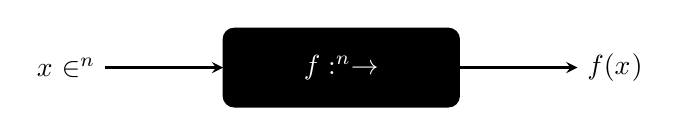
\begin{tikzpicture}
            \draw[rounded corners,fill] (0,0) rectangle (3,1);
            \node[text=white] at (1.5,0.5) {$\obj : \R^n \to \R$};
            \draw[-stealth,thick] (-1.5,0.5) -- (0,0.5);
            \node[left] at (-1.5,0.5) {$\iter \in \R^n$};
            \draw[-stealth,thick] (3,0.5) -- (4.5,0.5);
            \node[right] at (4.5,0.5) {$\obj(\iter)$};
        \end{tikzpicture}
    \end{center}

    \medskip
    
    \begin{block}{}
        \begin{enumerate}
            \item $f$ may be smooth, but derivatives \alert{cannot} be evaluated.
            \item Each function evaluation is \alert{expensive}.
            \item The measure of complexity is the number of \alert{function evaluations}.
            \item Do \alert{not} use DFO if any kind of first order information is available.
        \end{enumerate}
    \end{block}
\end{frame}

\begin{frame}
    \frametitle{Examples of DFO problems}

    \begin{enumerate}
        \item Automatic error analysis \parencite{Higham_1993,Higham_2002}
        \item Tuning nonlinear optimization methods \parencite{Audet_Orban_2006}
        \item \alert<2>{Hyperparameter tuning} \parencite{Ghanbari_Scheinberg_2017}
        \item Censored regression \parencite{Chen_Etal_2018}
        \item Aeroacoustic shape design \parencite{Marsden_2004,Marsden_Etal_2004}
        \item Computational fluid dynamics \parencite{Duvigneau_Visonneau_2004}
        \item \alert<2>{Aircraft engine engineering}~\parencite{Gazaix_Etal_2019}
        \item Rapid-cycling synchrotron accelerator modeling \parencite{Eldred_Etal_2022}
        \item \dots
    \end{enumerate}

    \medskip

    \pause
    \begin{block}{}
        In what follows, we detail two examples from \alert{machine learning} and \alert{MDO}.
    \end{block}
\end{frame}

\begin{frame}
    \frametitle{Hyperparameter tuning in machine learning}

    \begin{center}
        \begin{tikzpicture}
			\uncover<2>{
				\draw[rounded corners,pattern=north east lines,pattern color=DarkOrchid,fill opacity=0.3] (8,3) rectangle (11,4.5);
			}
			\draw[thick,rounded corners] (0,0) rectangle (3,1.5);
			\draw[thick,rounded corners] (0,4) rectangle (3,5.5);
			\draw[thick,rounded corners] (4,2) rectangle (7,3.5);
			\draw[thick,rounded corners] (8,1) rectangle (11,2.5);
			\draw[thick,rounded corners] (8,3) rectangle (11,4.5);
			\draw[thick,-stealth] (3,1) -- (5.5,1) -- (5.5,2);
			\draw[thick] (3,0.5) -- (7.5,0.5) -- (7.5,2.5) -- (7,2.5);
			\draw[thick,-stealth] (7.5,1.75) -- (8,1.75);
			\draw[thick] (3,4.75) -- (7.5,4.75) -- (7.5,3) -- (7,3);
			\draw[thick,-stealth] (7.5,3.75) -- (8,3.75);
			\node at (0.6,0.75) {\includegraphics[height=0.75cm]{images/ml/presentation.png}};
			\node at (0.6,4.75) {\includegraphics[height=0.75cm]{images/ml/search.png}};
			\node at (4.6,2.75) {\includegraphics[height=0.75cm]{images/ml/deep-learning.png}};
			\node at (8.6,1.75) {\includegraphics[height=0.75cm]{images/ml/analysis.png}};
			\node at (8.6,3.75) {\includegraphics[height=0.75cm]{images/ml/analytics.png}};
			\node at (2,0.75) {\makecell{Training\\ dataset}};
			\node at (2,4.75) {\makecell{Testing\\ dataset}};
			\node at (6,2.75) {\makecell{Machine\\ learning}};
			\node at (10,1.75) {\makecell{Training\\ accuracy}};
			\node at (10,3.75) {\makecell{Testing\\ accuracy}};
			\uncover<2>{
				\draw[rounded corners,pattern=north east lines,pattern color=DarkOrchid,fill opacity=0.3] (0,2) rectangle (3,3.5);
				\draw[thick,rounded corners] (0,2) rectangle (3,3.5);
				\draw[thick,-stealth] (3,2.75) -- (4,2.75);
				\node at (0.6,2.75) {\includegraphics[height=0.7cm]{images/ml/admin-panel.png}};
				\node at (2,2.75) {\makecell{Hyper-\\ parameters}};
			}
		\end{tikzpicture}
    \end{center}

    \pause
    \begin{block}{}
        \begin{enumerate}
            \item How to \alert{maximize} the testing accuracy by tuning the \alert{hyperparameters}?
            \item What is the \alert{gradient} of the testing accuracy?
        \end{enumerate}
    \end{block}
\end{frame}

\begin{frame}
    \frametitle{Aircraft engine pylon optimization}

    Where to position the engines to maximize the performance of an aircraft?

    \medskip
    
    \begin{center}
        \begin{tikzpicture}
            \draw[thick,rounded corners,pattern=north east lines,pattern color=DarkOrchid,fill opacity=0.3] (0,0) rectangle (3,1.5);
            \draw[thick,rounded corners] (-4,-2.5) rectangle (-1,-1);
            \draw[thick,rounded corners] (0,-2.5) rectangle (3,-1);
            \draw[thick,rounded corners] (4,-2.5) rectangle (7,-1);
            \draw[thick,dotted,rounded corners,DarkOrchid] (-4.25,-2.75) rectangle (7.25,-0.75);
			\draw[thick,stealth-stealth] (1.5,0) -- (1.5,-1);
			\draw[thick,stealth-stealth] (-2.5,-1) -- (-2.5,-0.5) -- (1,-0.5) -- (1,0);
			\draw[thick,stealth-stealth] (5.5,-1) -- (5.5,-0.5) -- (2,-0.5) -- (2,0);
            \node at (1.5,0.75) {\makecell{Multi-disciplinary\\ optimization}};
            \node at (-2.5,-1.75) {\makecell{Aerodynamic\\ optimization}};
            \node at (1.5,-1.75) {\makecell{OAD\\ optimization}};  % Overall Aircraft Design
            \node at (5.5,-1.75) {\makecell{Structure\\ optimization}};
            \node[below right,text=DarkOrchid] at (-4.25,-2.75) {\small\emph{Different independent disciplines/departments}};
        \end{tikzpicture}
    \end{center}
    
	\begin{block}{}
        \begin{enumerate}
            \item Each discipline provides only a \alert{fragment} of the problem.
            \item The derivatives of some or all components involved may be \alert{unknown}.
        \end{enumerate}
    \end{block}
\end{frame}

\begin{frame}
    \frametitle{A lack of theories and methodologies}

    We are in lack of
    \begin{enumerate}
        \item easily usable DFO \alert{solvers}, and
        \item \alert{theoretical} understanding of several DFO techniques.
    \end{enumerate}

    \bigskip

    \begin{block}{Organization of this thesis defense}
        In what follows, we will present
        \begin{enumerate}
            \item the \alert{PDFO} software, interfacing existing widely used methods,
            \item an investigation of a \alert{DFO mechanism} introduced by \textcite{Powell_2006},
            \item new developments in the \alert{SQP method} (derivative-based), and
            \item the \alert{COBYQA} method, a new DFO method.
        \end{enumerate}
    \end{block}
\end{frame}

\section{Solving DFO problems using PDFO}

\begin{frame}
    \frametitle{Existing methods for DFO}

    We want to solve
    \begin{equation*}
        \min_{\iter \in \fset \subseteq \R^n} \obj(\iter),
    \end{equation*}
    where derivatives of~$\obj$ (and possibly the constraint functions) are \alert{unknown}.

    \bigskip

    \begin{block}{}
        \begin{enumerate}
            \item \alert{Direct-search methods}: Nelder-Mead \parencite{Nelder_Mead_1965}, GPS \parencite{Booker_Etal_1999}, MADS \parencite{Audet_Dennis_2006}, \dots
            \item \alert{Model-based methods}: Wedge \parencite{Marazzi_Nocedal_2002}, GALAHAD \parencite{Gould_Orban_Toint_2003}, MNH \parencite{Wild_2008}, \textcite{Fasano_Morales_Nocedal_2009}, \textcite{Conejo_Karas_Pedroso_2015}, \textcite{Audet_Digabel_Peyrega_2016}, \textcite{Jarre_Lieder_2017}, \emph{Powell's methods}, \dots
            % UOBYQA \parencite{Powell_2002}, NEWUOA \parencite{Powell_2006}, BOBYQA \parencite{Powell_2009}, LINCOA \parencite{Powell_2015}, COBYLA \parencite{Powell_1994}, \dots
        \end{enumerate}
    \end{block}
    
	% \begin{enumerate}
    %     \item \textcite{Jarre_Lieder_2017}.
    %     \item \textcite{Santo_Denysiuk_Fernandes_2014}.
    %     \item \textcite{Audet_Digabel_Peyrega_2016}.
    %     \item \textcite{Conejo_Karas_Pedroso_2015}.
    %     \item \textcite{Gould_Orban_Toint_2003}.
    % \end{enumerate}
\end{frame}

\begin{frame}
    \frametitle{A focus on Powell's DFO solvers}
    
	Powell's designed five DFO solvers.

    \medskip

    \begin{center}
        \begin{tabular}{lll}
            \toprule
            Solver  & Feasible set~$\Omega$                                 & References\\
            \midrule
            UOBYQA  & $\R^n$                                                & \textcite{Powell_2002}\\
            NEWUOA  & $\R^n$                                                & \textcite{Powell_2006}\\
            BOBYQA  & $\set{x \in \R^n : \xl \le x \le \xu}$                & \textcite{Powell_2009}\\
            LINCOA  & $\set{x \in \R^n : A x \le b}$                        & \textcite{Powell_2015}\\
            COBYLA  & $\set{x \in \R^n : \con[i](x) \ge 0, ~ i \in \iub}$   & \textcite{Powell_1994}\\
            \bottomrule
        \end{tabular}
    \end{center}

    \medskip

    \begin{block}{An obstacle to using Powell’s DFO solvers}
        Powell implemented them in \alert{Fortran 77}\dots
    \end{block}
\end{frame}

\begin{frame}
    \frametitle{The need for PDFO}

    \begin{block}{}
        \alert{PDFO} is a \alert{cross-platform} package interfacing Powell's DFO solvers.
    \end{block}

    \medskip

    \begin{enumerate}
        \item The \alert{MATLAB} signature is consistent with \texttt{fmincon}.
        \item The \alert{Python} signature is consistent with \texttt{scipy.optimize.minimize}.
        \item PDFO is \alert{open-source} and distributed under the LGPLv3+ license.
        \item This is \alert{not} a reimplementation of Powell's solvers.
    \end{enumerate}

    \medskip
    
	\begin{center}
        \href{https://www.pdfo.net/}{\includegraphics[width=0.8in]{images/qr/pdfo.png}}

        \scriptsize\url{https://www.pdfo.net/}
    \end{center}
\end{frame}

\begin{frame}
    \frametitle{Numerical experiments using PDFO}
    
	\begin{columns}
        \begin{column}{0.45\textwidth}
            We compare the solvers
            \begin{enumerate}
                \item on \alert{unconstrained} problems,
                \item from the \alert{CUTEst} set,
                \item of dimension \alert{at most 50}\only<1>{.}\only<2>{,}
                \uncover<2>{
                    \item replacing~$\obj$ with
                    \begin{equation*}
                        \tilde{\obj}(\iter) = [1 + \epsilon(\iter)] \obj(\iter),
                    \end{equation*}
                    with~$\epsilon(x) \sim N(0, \sigma^2)$,~$\sigma = 10^{-2}$.
                }
            \end{enumerate}
        \end{column}
        \begin{column}{0.55\textwidth}
            \begin{center}
                \only<1>{\drawperformanceprofiles{{"NEWUOA","BOBYQA","LINCOA","COBYLA"}}{plain-1-50-perf-newuoa-bobyqa-lincoa-cobyla-u.csv}{4}}%
                \only<2>{\drawperformanceprofiles{{"NEWUOA","BOBYQA","LINCOA","COBYLA"}}{noisy-1-50-2-perf-newuoa-bobyqa-lincoa-cobyla-u.csv}{1}}
            \end{center}
        \end{column}
    \end{columns}
\end{frame}

\section{Understanding a DFO mechanism}

\begin{frame}
    \frametitle{A model-based DFO mechanism}
    
    \begin{block}{}
        Many model-based DFO methods \alert{approximate}~$\obj$ by some quadratic~$\objm[k]$ with
        \begin{equation*}
            \objm[k](y) = \obj(y), ~ y \in \xpt[k],
        \end{equation*}
        for some~$\xpt[k] \subseteq \R^n$, \alert{updated} iteratively.
        How to \alert{choose}~$\xpt[0]$?
    \end{block}

    \smallskip

    \begin{columns}
        \begin{column}{0.6\textwidth}
            As \textcite{Powell_2006}, assuming that~$\iter[0] = 0$, let
            \begin{empheq}[left={z^j = \empheqlbrace}]{alignat*=2}
                & \textcolor{OliveGreen}{0}                 && \quad \text{if~$j = 1$,}\\
                & \textcolor{BurntOrange}{\delta e_{j - 1}} && \quad \text{if~$2 \le j \le n + 1$,}\\
                & \textcolor{Maroon}{-\delta e_{j - n - 1}} && \quad \text{if~$n + 2 \le j \le 2n + 1$,}
            \end{empheq}
            for some~$\delta > 0$, and \alert{define}~$\xpt[0]$ to be
            \begin{equation*}
                \mathcal{Z}_m = \set{z^1, z^2, \dots, z^m},
            \end{equation*}
            for some~$m \le 2n + 1$.
        \end{column}
        \begin{column}{0.4\textwidth}
            \begin{center}
                \begin{tikzpicture}
                    \begin{axis}[
                        axis equal image,
                        xtick={-1,0,1},
                        ytick={-1,0,1},
                        xticklabels={$-\delta$,$0$,$\delta$},
                        yticklabels={$-\delta$,$0$,$\delta$},
                        xlabel={$x_1$},
                        ylabel={$x_2$},
                        width=\columnwidth,
                    ]
                        \addplot[only marks,mark options={fill=OliveGreen}] coordinates {(0, 0)} node[above right,text=OliveGreen] {$z^0$};
                        \addplot[only marks,mark options={fill=BurntOrange}] coordinates {(1, 0)} node[above,text=BurntOrange] {$z^1$};
                        \addplot[only marks,mark options={fill=BurntOrange}] coordinates {(0, 1)} node[right,text=BurntOrange] {$z^2$};
                        \addplot[only marks,mark options={fill=Maroon}] coordinates {(-1, 0)} node[above,text=Maroon] {$z^3$};
                        \addplot[only marks,mark options={fill=Maroon}] coordinates {(0, -1)} node[right,text=Maroon] {$z^4$};
                        \addplot[no marks] coordinates{(0, 0) (1, 0)};
                        \addplot[no marks] coordinates{(0, 0) (0, 1)};
                        \addplot[no marks] coordinates{(0, 0) (-1, 0)};
                        \addplot[no marks] coordinates{(0, 0) (0, -1)};
                    \end{axis}  
                \end{tikzpicture}
            \end{center}
        \end{column}
    \end{columns}
\end{frame}

\begin{frame}
    \frametitle{$\Lambda$-poisedness of interpolation set}

    We assume that~$\objm[k]$ solves
    \begin{align*}
        \min_{Q}    & \quad \norm{H_{\text{old}} - \nabla^2 Q}_{\mathsf{F}}\\
        \text{s.t.} & \quad Q(y) = \obj(y), ~ y \in \xpt[k],
    \end{align*}
    for some~$H_{\text{old}} \in \R^{n \times n}$ (e.g.,~$0$ or~$\nabla^2 \objm[k - 1]$).
    
    \medskip

    \begin{block}{}
        We denote
        \begin{enumerate}
            \item $\xpt[k] = \set{y^1, y^2, \dots, y^m}$,
            \item $\mathcal{C} \subseteq \R^n$ any compact set, and
            \item $\lagp[i]$ the (quadratic) \alert{Lagrange polynomial} associated with~$y^i$, solving
            \begin{align*}
                \min_{Q}    & \quad \norm{\nabla^2 Q}_{\mathsf{F}}\\
                \text{s.t.} & \quad Q(y^j) = \delta_{i, j}, ~ j \in \set{1, 2, \dots, m}.
            \end{align*}
        \end{enumerate}
    \end{block}
\end{frame}

\begin{frame}
    \frametitle{$\Lambda$-poisedness of interpolation set (cont'd)}

    \textcite{Ciarlet_Raviart_1972} and \textcite{Powell_2001} show that
    \begin{equation*}
        \max_{\iter \in \mathcal{C}} @@ \abs{\obj(\iter) - \objm[k](\iter)} \le \frac{m \theta_{\mathcal{C}} \Lambda_{\mathcal{C}}}{6} \max_{1 \le i \le m} \max_{\iter \in \mathcal{C}} @@ \norm{\iter - y^i}^3,
    \end{equation*}
    where
    \begin{equation*}
        \theta_{\mathcal{C}} = \max_{\iter \in \mathcal{C}} @@ \norm{\nabla^3 \obj(\iter)} \quad \text{and} \quad \Lambda_{\mathcal{C}} = \max_{1 \le i \le m} \max_{\iter \in \mathcal{C}} @@ \abs{\lagp[i](\iter)}.
    \end{equation*}

    \begin{block}{$\Lambda$-poisedness \parencite{Conn_Scheinberg_Vicente_2009b}}
        The set~$\xpt[k]$ is \alert{$\Lambda$-poised} in~$\mathcal{C} \subseteq \R^n$ if~$\lambda \ge \Lambda_{\mathcal{C}}$.
    \end{block}
    
    \medskip

    \begin{block}{}
        \begin{enumerate}
            \item If~$\xpt[k] \subseteq \mathcal{C}$, then~$\Lambda_{\mathcal{C}} \ge 1$.
            \item The lower~$\Lambda_{\mathcal{C}}$ is, the better~$\xpt[k]$ is.
        \end{enumerate}
    \end{block}
\end{frame}

\begin{frame}
    \frametitle{Bounds for the~$\Lambda$-poisedness of~$\mathcal{Z}_m$}

    \begin{block}{}
        For any~$p \in [1, \infty)$,~$\mathcal{Z}_m$ is~\alert{$\Lambda_p$-poised} in~$\mathcal{B}_p(\delta) = \set{\iter \in \R^n : \norm{\iter}_p \le \delta}$ for some
        \begin{equation*}
            \Lambda_p \in \big[ 1 + (2n + 1 - m)^{\frac{p - 1}{p}},  n \big],
        \end{equation*}
        where~$0^0 = 0$.
        Moreover, the lower bound is \alert{reached} if~$p \in \set{1, 2}$.
    \end{block}

    \only<1>{
        \bigskip

        \begin{center}
            \begin{tikzpicture}
                \begin{axis}[
                    xtick={22,41},
                    xticklabels={$n + 2$,$2n + 1$},
                    ytick={1,3,5,7,9},
                    xlabel={$m$ (with~$n = 20$)},
                    ylabel={Lower bound},
                    width=0.9\textwidth,
                    height=0.55\textheight,
                    samples at={22,...,41},
                ]
                    \addplot{ifthenelsefpu((x==41), 1, 2)};
                    \addplot{1+(41-x)^(1/2)};
                    \addplot{1+(41-x)^(2/3)};
                    \addplot{1+(41-x)^(3/4)};
                    \addlegendentry{$p = 1$}
                    \addlegendentry{$p = 2$}
                    \addlegendentry{$p = 3$}
                    \addlegendentry{$p = 4$}
                \end{axis}  
            \end{tikzpicture}
        \end{center}
    }
    \only<2>{
        \emph{Proof of concept}.
        \begin{enumerate}
            \item Construct explicit formulae for~$\set{\lagp[i]}_{1 \le i \le m}$.
            \item Show that~$\mathcal{Z}_m$ is~$\Lambda_p$-poised in~$\mathcal{B}_p(\delta)$ with
            \begin{equation*}
                \Lambda_p = \max_{\iter \in \mathcal{B}_p(\delta)} \abs{\lagp[1](\iter)}.
            \end{equation*}
            \item The lower bound is obtained by evaluating~$\abs{\lagp[1](\iter)}$ at a particular~$\iter$.
            \item The upper bound follows~$\mathcal{B}_p(\delta) \subseteq \mathcal{B}_{\infty}(\delta)$ so that~$\Lambda_p \le \Lambda_{\infty}$ with
            \setlength{\belowdisplayskip}{0pt}
            \begin{equation*}
                \Lambda_{\infty} = \max \set{2n + 2 - m, n - 1}.
            \end{equation*}
        \end{enumerate}
    }
\end{frame}

\begin{frame}
    \frametitle{A special case and its significance}

    \begin{block}{}
        For any~$p \in [1, \infty)$, then~$\mathcal{Z}_{2n + 1}$ is~$\Lambda_p$-poised in~$\mathcal{B}_p(\delta)$ with
        \begin{equation*}
            \Lambda_p = \max \set[\big]{1, n^{\frac{p - 2}{2}} - 1}.
        \end{equation*}
    \end{block}

    \medskip

    We then remark the following
    \begin{enumerate}
        \item For~$p \in [1, 2]$, we have~$\Lambda_p = 1$.
        \item Since~$\mathcal{Z}_m \subseteq \mathcal{B}_p(\delta)$,~$\mathcal{Z}_m$ is \alert{at best}~$1$-poised in~$\mathcal{B}_p(\delta)$.
    \end{enumerate}
    
    \medskip

    \begin{block}{}
        Therefore,~$m = 2n + 1$ is \alert{optimal} for~$\mathcal{Z}_m$ when~$p \in [1, 2]$.
    \end{block}

    \medskip

    \begin{enumerate}
        \item We \alert{conjecture} that this is true for all~$p \in [1, \infty)$.
        \item It provides a theoretical \alert{understanding} of Powell's default value.
    \end{enumerate}
\end{frame}

\section{New developments in the SQP method}

\begin{frame}
    \frametitle{The problem}

	We consider in what follows
    \begin{align*}
        \min_{\iter \in \R^n}   & \quad \obj(\iter)\\
        \text{s.t.}             & \quad \con(\iter) \le 0,
    \end{align*}
    where derivatives of~$\obj$ and~$\con$ are \alert{known}.
    Recall that its \alert{Lagrangian} is
    \begin{equation*}
        \lag(\iter, \lm) = \obj(\iter) + \lm^{\T} \con(\iter).
    \end{equation*}

    \begin{block}{The purpose of the SQP method}
        How to \alert{practically} and \alert{efficiently} (Q-quadratically) solve this problem?
    \end{block}
\end{frame}

\begin{frame}
    \frametitle{The Sequential Quadratic Programming (SQP) method}
    
	Given an iterate~$\iter[k] \in \R^n$, let~$\step[k]$ be an approximate solution to
    \begin{align*}
        \min_{\step \in \R^n}   & \quad \nabla \obj(\iter[k])^{\T} \step + \frac{1}{2} \step^{\T} \nabla_{x, x}^2 \lag(\iter[k], \lm[k]) \step\\
        \text{s.t.}             & \quad \con(\iter[k]) + \nabla \con(\iter[k]) \step \le 0,
    \end{align*}
    for some~$\lm[k]$ and set~$\iter[k + 1] = \iter[k] + \step[k]$.
    
    \medskip

    \begin{block}{}
        \begin{enumerate}
            \item It generalizes the \alert{Sequential Linear Programming} (SLP) method.
            \item It is close to a \alert{Newton-Raphson} step for the KKT system.
            \item It does not work if~$\nabla_{x, x}^2 \lag(\iter[k], \lm[k])$ is replaced with~$\nabla^2 \obj(\iter[k])$.
        \end{enumerate}
    \end{block}
\end{frame}

\begin{frame}
    \frametitle{A new interpretation of the SQP subproblem}
    
	\begin{enumerate}
        \item Assume for simplicity that the problem's constraints are~$\con(\iter) = 0$.
        \item For some~$\bar{\iter}$ and~$\bar{\lm}$, define
        \begin{equation*}
            Q(\step) = \obj(\bar{\iter}) + \nabla \obj(\bar{\iter})^{\T} \step + \frac{1}{2} \step^{\T} \only<1>{\textcolor{OliveGreen}{\nabla_{x, x}^2 \lag(\bar{\iter}, \bar{\lm})}}\only<2>{\textcolor{BurntOrange}{\nabla^2 \obj(\bar{\iter})}} \step.
        \end{equation*}
    \end{enumerate}

    \begin{block}{}
        Consider a curve parametrized by~$\iter : \R \to \R^n$ satisfying
        \begin{equation*}
            c\big(\iter(t)\big) = c(\bar{\iter}) \quad \text{for all~$t \in \R$}, \quad \text{and} \quad \iter(0) = \bar{\iter}.
        \end{equation*}
        Under some regularity assumptions, there exist~$\nu \ge 0$ and~$\epsilon > 0$ such that
        \begin{equation*}
            \abs[\big]{\obj\big(\iter(t)\big) - Q\big(\iter'(0) t\big)} \le \bigg(\nu t + \frac{1}{2} \abs[\big]{\iter''(0)^{\T} \only<1>{\textcolor{OliveGreen}{\big[\nabla \obj(\bar{\iter}) + \nabla c(\bar{\iter})^{\T} \bar{\lm} \big]}}\only<2>{\textcolor{BurntOrange}{\nabla \obj(\bar{\iter})}}} \bigg) t^2,
        \end{equation*}
        for all~$t \in (-\epsilon, \epsilon)$.
    \end{block}
\end{frame}

\begin{frame}
    \frametitle{The trust-region SQP method}
    
	\begin{block}{}
        \begin{enumerate}
            \item The convergence properties of the SQP method are \alert{local}.
            \item We employ the trust-region framework as a globalization strategy.
        \end{enumerate}
    \end{block}

    Given an iterate~$\iter[k] \in \R^n$, let~$\step[k]$ be an approximate solution to
    \begin{align*}
        \min_{\step \in \R^n}   & \quad \nabla \obj(\iter[k])^{\T} \step + \frac{1}{2} \step^{\T} \nabla_{x, x}^2 \lag(\iter[k], \lm[k]) \step\\
        \text{s.t.}             & \quad \con(\iter[k]) + \nabla \con(\iter[k]) \step \le 0,\\
                                & \quad \norm{\step} \le \rad[k],
    \end{align*}
    for some~$\lm[k]$ and~$\rad[k] > 0$.
    Given a merit function~$\merit$, we then set
    \begin{empheq}[left={\iter[k + 1] = \empheqlbrace}]{alignat*=2}
        & \iter[k] + \step[k]   && \quad \text{if~$\merit(\iter[k] + \step[k]) < \merit(\iter[k])$,}\\
        & \iter[k]              && \quad \text{otherwise.}
    \end{empheq}

    \pause
    How to \alert{solve} the subproblem?
    What if it is \alert{infeasible}?
\end{frame}

\begin{frame}
    \frametitle{The \citeauthor{Vardi_1985} approach}

    To define the \alert{trial step}~$\step[k]$,
    \begin{enumerate}
        \item we \alert{shift} the infeasible linear constraints towards~$x^k$, and
        \item we evaluate~$\step[k]$ on the \alert{relaxed subproblem}.
    \end{enumerate}
    
	\begin{columns}
        \begin{column}{0.45\textwidth}
            \begin{center}
                \begin{tikzpicture}
                    % Linear constraints
                    \uncover<1>{\fill[color=RoyalBlue,opacity=0.4] (-4,-1) -- (-1.5,-1) -- (-0.5,4) -- (-4,4) -- cycle;}
                    \uncover<2->{\fill[color=RoyalBlue,opacity=0.4] (-4,-1) -- (-1.175,-1) -- (-0.175,4) -- (-4,4) -- cycle;}
                    \uncover<1>{\fill[color=RoyalBlue,opacity=0.4] (-4,1) -- (0,4) -- (-4,4) -- cycle;}
                    \uncover<2->{\fill[color=RoyalBlue,opacity=0.4] (-4,0) -- (1,3.75) -- (1,4) -- (-4,4) -- cycle;}
        
                    % Trust regions
                    \begin{scope}
                        \clip (-4,-1) rectangle (1,4);
                        \draw[fill=Dandelion,opacity=0.7] (0,0) circle (3);
                    \end{scope}
        
                    % Feasible region for the relaxed subproblem
                    \begin{scope}
                        \clip (-4,0) -- (-15/34,363/136) -- (-0.175,4) -- (-4,4) -- cycle;
                        \uncover<3->{\fill[pattern=north west lines,opacity=0.7] (0,0) circle (3);}
                    \end{scope}
        
                    % Frame and annotations
                    \uncover<4>{
                        \draw[-stealth,thick] (0,0) -- (-0.9,2.7);
                        \node[above right] at (-0.45,1.35) {$\step[k]$};
                    }
                    \draw[fill] (0,0) circle (1.4pt) node[below right] {$\iter[k]$};
                    \draw[thick] (-4,-1) rectangle (1,4);
                \end{tikzpicture}
            \end{center}
        \end{column}
        \begin{column}{0.55\textwidth}
            \begin{tikzpicture}
                \draw[fill=Dandelion,opacity=0.7] (0,0) circle (.2);
                \node[right] at (.4,0) {Trust region};
                \fill[color=RoyalBlue,opacity=0.4] (-.2,-0.8) rectangle (.2,-0.4);
                \node[right] at (.4,-0.6) {Linear constraints};
                \uncover<3->{
                    \fill[pattern=north west lines,opacity=0.7] (-.2,-1.4) rectangle (.2,-1);
                    \node[right] at (.4,-1.2) {Feasible region for~$\step[k]$};
                }
            \end{tikzpicture}
        \end{column}
    \end{columns}
\end{frame}

\begin{frame}
    \frametitle{The \citeauthor{Vardi_1985} approach (cont'd)}

    The subproblem becomes
    \begin{align*}
        \min_{\step \in \R^n}   & \quad \nabla \obj(\iter[k])^{\T} \step + \frac{1}{2} \step^{\T} \nabla_{x, x}^2 \lag(\iter[k], \lm[k]) \step\\
        \text{s.t.}             & \quad \Gamma \con(\iter[k]) + \nabla \con(\iter[k]) \step \le 0,\\
                                & \quad \norm{\step} \le \rad[k],
    \end{align*}
    where~$\Gamma$ is the diagonal matrix such that
    \begin{empheq}[left={\Gamma_{i, i} = \empheqlbrace}]{alignat*=2}
        & \alpha    && \quad \text{if~$\con[i](\iter[k]) > 0$,}\\
        & 1         && \quad \text{otherwise,}
    \end{empheq}
    with~$\alpha \in [0, 1]$ being chosen to make the subproblem \alert{feasible}.

    \smallskip
    
    \begin{block}{}
        \begin{enumerate}
            \item The original idea is due to \textcite{Vardi_1985}.
            \item This version \alert{adapts} an idea from \textcite{Powell_1978a}.
        \end{enumerate}
    \end{block}
\end{frame}

\begin{frame}
    \frametitle{The \citeauthor{Byrd_1987}-\citeauthor{Omojokun_1989} approach}

    To define the \alert{trial step}~$\step[k]$, we decompose~$\step[k] = \nstep[k] + \tstep[k]$, where
    \begin{enumerate}
        \item the \alert{normal step}~$\nstep[k]$ reduces the (possible) constraint violation, and
        \item the \alert{tangential step}~$\tstep[k]$ reduces the objective function of the subproblem.
    \end{enumerate}
    
    \begin{columns}
        \begin{column}{0.45\textwidth}
            \begin{center}
                \begin{tikzpicture}
                    % Linear constraints
                    \uncover<1-6>{\fill[color=RoyalBlue,opacity=0.4] (-4,-1) -- (-1.5,-1) -- (-0.5,4) -- (-4,4) -- cycle;}
                    \uncover<7>{\fill[color=RoyalBlue,opacity=0.4] (-4,-1) -- (-2.1,-1) -- (-1.1,4) -- (-4,4) -- cycle;}
                    \uncover<1,2>{\fill[color=RoyalBlue,opacity=0.4] (-4,1) -- (0,4) -- (-4,4) -- cycle;}
                    \uncover<3->{\fill[color=RoyalBlue,opacity=0.4] (-4,0.125) -- (1,3.875) -- (1,4) -- (-4,4) -- cycle;}
        
                    % Trust regions
                    \begin{scope}
                        \clip (-4,-1) rectangle (1,4);
                        \draw[fill=Dandelion,draw opacity=0.7,fill opacity=0.5] (0,0) circle (3);
                        \draw[densely dotted,fill=Dandelion,opacity=0.7] (0,0) circle (2.5);
                    \end{scope}
        
                    % Feasible region for the tangential subproblem
                    \begin{scope}
                        \clip (-4,0.125) -- (-27/34,43/17) -- (-0.5,4) -- (-4,4) -- cycle;
                        \uncover<4-6>{\fill[pattern=north west lines,opacity=0.7] (0,0) circle (3);}
                    \end{scope}
                    \begin{scope}
                        \clip (-4,0.125) -- (-1.5,2) -- (-1.1,4) -- (-4,4) -- cycle;
                        \uncover<7>{\fill[pattern=north west lines,opacity=0.7] (0,0) circle (3);}
                    \end{scope}
        
                    % Frame and annotations
                    \uncover<5>{
                        \draw[-stealth,thick,OliveGreen] (-1.5,2) -- (-0.9,2.7);
                        \node[below,xshift=5pt,text=OliveGreen] at (-1.2,2.35) {$\tstep[k]$};
                        \draw[-stealth,thick] (0,0) -- (-0.9,2.7);
                        \node[above right] at (-0.45,1.35) {$\step[k]$};
                    }
                    \uncover<2->{
                        \draw[-stealth,thick,Mahogany] (0,0) -- (-1.5,2);
                        \node[below left,text=Mahogany] at (-0.75,1) {$\nstep[k]$};
                    }
                    \draw[fill] (0,0) circle (1.4pt) node[below right] {$\iter[k]$};
                    \draw[thick] (-4,-1) rectangle (1,4);
                \end{tikzpicture}
            \end{center}
        \end{column}
        \begin{column}{0.55\textwidth}
            \begin{tikzpicture}
                \draw[fill=Dandelion,draw opacity=0.7,fill opacity=0.5] (0,0) circle (.2);
                \node[right] at (.4,0) {Trust region};
                \draw[densely dotted,fill=Dandelion,opacity=0.7] (0,-0.6) circle (.2);
                \node[right] at (.4,-0.6) {Reduced trust region};
                \fill[color=RoyalBlue,opacity=0.4] (-.2,-1.4) rectangle (.2,-1);
                \node[right] at (.4,-1.2) {Linear constraints};
                \uncover<4->{
                    \fill[pattern=north west lines,opacity=0.7] (-.2,-2) rectangle (.2,-1.6);
                    \node[right] at (.4,-1.8) {Feasible region for~$\tstep[k]$};
                }
            \end{tikzpicture}

            \bigskip

            Our \alert<1-6>{new} approach vs. the \alert<7>{standard}\footfullcite{Conn_Gould_Toint_2000} one.
        \end{column}
    \end{columns}
\end{frame}

\begin{frame}
    \frametitle{The \citeauthor{Byrd_1987}-\citeauthor{Omojokun_1989} approach (cont'd)}

    The normal step~$\nstep[k]$ solves approximately
    \begin{align*}
        \min_{\step \in \R^n}   & \quad \norm[\big]{\posp{\con(\iter[k]) + \nabla \con(\iter[k]) \step}},\\
        \text{s.t.}             & \quad \norm{\step} \le \zeta \rad[k],
    \end{align*}
    for some~$\zeta \in (0, 1)$ and the tangential step~$\tstep[k]$ solves approximately
    \begin{align*}
        \min_{\step \in \R^n}   & \quad \big[ \nabla \obj(\iter[k]) + \nabla_{x, x}^2 \lag(\iter[k], \lm[k]) \nstep[k] \big]^{\T} \step + \frac{1}{2} \step^{\T} \nabla_{x, x}^2 \lag(\iter[k], \lm[k]) \step\\
        \text{s.t.}             & \quad \nabla \con(\iter[k])^{\T} \step \le \only<1>{\textcolor{OliveGreen}{\negp{- \con(\iter[k]) - \nabla \con(\iter[k]) \nstep[k]}}}\only<2>{\textcolor{BurntOrange}{0}},\\
                                & \quad \norm{\nstep[k] + \step} \le \rad[k].
    \end{align*}
    
    \begin{block}{}
        \begin{enumerate}
            \item The original idea is due to \textcite{Byrd_1987} and \textcite{Omojokun_1989}.
            \item This is \only<1>{our \textcolor{OliveGreen}{\textbf{new}}}\only<2>{the \textcolor{BurntOrange}{\textbf{standard}}} approach.
        \end{enumerate}
    \end{block}
\end{frame}

% \begin{frame}
%     \frametitle{A connection between the two approaches}
    
% 	To do.
% \end{frame}

\section{Our new DFO method COBYQA}

\begin{frame}
    \frametitle{The problem addressed by our new DFO method}
    
	We design a method named COBYQA to solve
    \begin{align*}
        \min_{x \in \R^n}   & \quad \obj(x)\\
        \text{s.t.}         & \quad \con(x) \le 0,\\
                            & \quad \xl \le x \le \xu,
    \end{align*}
    where derivatives of~$\obj$ and~$\con$ are \alert{unknown}.

    \medskip

    \begin{block}{}
        \begin{enumerate}
            \item The method also accepts equality constraints.
            \item The bound constraints are handled separately.
            \item Our goal is to design a \alert{successor} for COBYLA.
            \item We want to release a stable \alert{implementation} of COBYQA.
        \end{enumerate}
    \end{block}
\end{frame}

\begin{frame}
    \frametitle{Inviolable bound constraints}
    
	\begin{block}{}
        We assume that the bound constraints~$\xl \le x \le \xu$ are \alert{inviolable}.
        \begin{enumerate}
            \item $f$ and/or~$\con$ may \alert{not} be defined otherwise.
            \item COBYQA must \alert{always} respect the bound constraints.
        \end{enumerate}
    \end{block}

    \bigskip

    This is the case for the two examples of DFO problem we detailed.
    \begin{enumerate}
        \item Hyperparameters in machine learning often admit inviolable bounds.
        \item Aircraft engine pylons must be beneath the wings.
    \end{enumerate}

    \bigskip

    \begin{block}{}
        COBYQA also handles \alert{linear constraints} separately.
    \end{block}
\end{frame}

\begin{frame}
    \frametitle{Interpolation-based quadratic models}
    
	COBYQA models~$\obj$ (and~$\con$) by \alert{quadratic} interpolation.

    \medskip

    \begin{block}{Derivative-free symmetric Broyden update}
        The~$k$th model~$\objm[k]$ of~$\obj$ solves
        \begin{align*}
            \min_{Q}    & \quad \norm[\big]{\nabla^2 \objm[k - 1] - \nabla^2 Q}_{\mathsf{F}}\\
            \text{s.t.} & \quad Q(y) = \obj(y), ~ y \in \xpt[k],
        \end{align*}
        where~$\objm[-1] = 0$ and~$\xpt[k] \subseteq \R^n$ satisfies
        \begin{equation*}
            n + 2 \le \card(\xpt[k]) \le \frac{1}{2} (n + 1) (n + 2).
        \end{equation*}
    \end{block}

    \medskip

    Similarly, we denote the~$k$th model of~$\con$ by~$\conm[k]$.
\end{frame}

\begin{frame}
    \frametitle{The derivative-free trust-region SQP method}

    Given an iterate~$\iter[k] \in \R^n$, our \alert{trust-region} subproblem is
    \begin{align*}
        \min_{\step \in \R^n}   & \quad \nabla \objm[k](\iter[k])^{\T} \step + \frac{1}{2} \step^{\T} \nabla_{x, x}^2 \lagm[k](\iter[k], \lm[k]) \step\\
        \text{s.t.}             & \quad \conm[k](\iter[k]) + \nabla \conm[k](\iter[k]) \step \le 0,\\
                                & \quad \norm{\step} \le \rad[k],
    \end{align*}
    for some~$\lm[k]$ and~$\rad[k] > 0$, where~$\lagm[k](\iter, \lm) = \objm[k](\iter) + \lm^{\T} \conm[k](\iter)$.

    \medskip

    \begin{block}{}
        \begin{enumerate}
            \item The subproblem is solved using our \alert{Byrd-Omojokun} approach.
            \item Usually,~$\iter[k] + \step[k]$ replaces a point in~$\xpt[k]$ to build~$\xpt[k + 1]$.
            \item When necessary, the \alert{geometry} of~$\xpt[k + 1]$ is improved.
            \item A lot of \alert{difficulties} are hidden here\dots
        \end{enumerate}
    \end{block}
\end{frame}

\begin{frame}
    \frametitle{Our Python implementation}

    We implemented COBYQA in \alert{Python} and made it \alert{publicly available}.
    
	\begin{center}
        \href{https://www.cobyqa.com/}{\includegraphics[width=0.8in]{images/qr/cobyqa.png}}

        \scriptsize\url{https://www.cobyqa.com/}
    \end{center}

    \begin{block}{}
        \textcite{Powell_2006} wrote
        \begin{quote}
            \enquote{The development of NEWUOA has taken nearly three years. The work was very frustrating [...]}
        \end{quote}
        We felt similar exasperation when developing COBYQA.
    \end{block}

    It will be included in
    \begin{enumerate}
        \item PDFO as a successor for COBYLA.
        \item GEMSEO, industrial software package for MDO (from IRT Saint-Exup{\'{e}}ry).
    \end{enumerate}
\end{frame}

\begin{frame}
    \frametitle{Comparison with existing DFO solvers}
    
	To do.
\end{frame}

\section{Conclusion and future research directions}

\begin{frame}
    \frametitle{Conclusion and future research directions}

	To do.
\end{frame}

\appendix

\begin{frame}[t,allowframebreaks]
    \frametitle{References}

	\printbibliography
\end{frame}

\end{document}